% based on a template made by the university of cologne
% http://www.mi.uni-koeln.de/wp-MIEDV/wp-content/uploads/2016/07/LaTeX-Vorlage.zip - 2023-11-02
\documentclass[12pt,a4paper]{scrartcl}

\addtokomafont{sectioning}{\rmfamily}
\usepackage[ngerman]{babel}% deutsches Sprachpaket wird geladen
\usepackage[T1]{fontenc} % westeuropäische Codierung wird verlangt
\usepackage[utf8]{inputenc}% Umlaute werden erlaubt
\usepackage[usenames]{color} % Erlaubt die Benutzung der namen im Farbpaket und deren Änderung
\usepackage{amsmath} % Erweiterung für den Mathe-Satz
\usepackage{amssymb} % alle Zeichen aus msam und msmb werden dargestellt
\usepackage{graphicx} % Graphiken und Bilder können eingebunden werden
%\usepackage{multirow} % erlaubt in einer Spalte einer Tabelle die Felder in mehreren Zeilen zusammenzufassen
\usepackage{enumerate} % erlaubt Nummerierungen
\usepackage{xurl} % Dient zur Auszeichnung von URLs; setzt die Adresse in Schreibmaschinenschrift.
\usepackage[center]{caption}  % Bildunterschrift wird zentriert
%\usepackage{subfigure} % mehrere Bilder können in einer fugure-Umgebung verwendet werden
%\usepackage{longtable} % Diese Umgebung ist ähnlich definiert wie die tabular-Umgebung, erlaubt jedoch mehrseitige Tabellen.
%\usepackage{paralist} % Modifikation der bereits bestehenden Listenumgebungen
\usepackage{lmodern}% Für die Schrift
\usepackage[hidelinks]{hyperref} % Links und Verweise werden innerhalb von PDF Dokumenten erzeugt
%\usepackage{wrapfig} % Das Paket ermöglicht es von Schrift umflossene Bilder und Tabellen einzufügen.
\usepackage{latexsym} % LaTeX-Symbole werden geladen
\usepackage{tikz} % Erlaubt es mit tikz zu zeichnen
\usepackage{tabularx} % Erlaubt Tabellen
\usepackage{algorithm} % Erlaubt Pseudocode
\usepackage{color} % Farbpaket wird geladen
%\usepackage{stmaryrd} % St Mary Road Symbole werden geladen
\usepackage{physics}
\usepackage{mhchem} % Chemie: \ce & \pu

\numberwithin{equation}{section} % Nummerierungen der Gleichungen, die durch equation erstellt werden, sind gebunden an die section
\newcommand{\HRule}{\rule{\linewidth}{0.7mm}}
\newcommand{\pu}[1]{\ensuremath{\mathrm{#1}}}

\hypersetup{
  pdftitle={B 3.3},
  pdfcreator={LaTeX via pandoc}}
  
  \hyphenation{Ener-gie-stragg-ling}

\setcounter{secnumdepth}{6}
\setcounter{tocdepth}{6}

\begin{document}
\begin{titlepage}
	\pagestyle{empty}

	\begin{center}

	\textsc{\LARGE Universität zu Köln }\\ [0.4cm]
	\textsc{Mathematisch-Naturwissenschaftliche Fakultät} \\[1.5cm]

	\includegraphics[width=0.45\textwidth]{../media/uni.jpg}\\[1.5cm]  % Uni-Logo wird geladen

	\textsc{\Large Praktikum~B}\\[2mm]
	\textsc{}\\[10mm]
	\HRule \\[0.4cm]

		{	\Huge \bfseries B 3.3}\\[0.4cm]
			{	\huge \bfseries Reichweite von $\pmb{\alpha}$-Strahlen}\\[0.3cm]
	
	\HRule \\[3cm]

		\textsc{\Large Catherine Tran } \\[3pt]
		\textsc{\Large Carlo Kleefisch } \\[3pt]
		\textsc{\Large Oliver Filla } \\[3pt]
		

	\end{center}
\end{titlepage}

\newpage
\tableofcontents
\newpage

\hypertarget{einleitung}{%
\section{Einleitung}\label{einleitung}}

In diesem Versuch wird die Wechselwirkung von $\alpha$-Teilchen mit den Elektronen der Atomhülle und der damit verbundene Abbremsung durch inelastische Stöße untersucht. Des Weiteren werden das Phänomen des $\alpha$-Zerfalls, Bremsvermögen, Reichweite in Luft und Folie sowie Energie-Straggling durch die Aufnahme von $\alpha$-Spektren mithilfe eines Sperrschichtdetektors studiert.

\hypertarget{theoretische-grundlagen}{%
\section{Theoretische Grundlagen}\label{theoretische-grundlagen}}

\hypertarget{alpha-zerfall}{%
\subsection{\texorpdfstring{$\alpha$-Zerfall}{\textbackslash alpha-Zerfall}}\label{alpha-zerfall}}

Der $\alpha$-Zerfall ist eine Form des radioaktiven Zerfalls, bei dem ein Heliumkern $\ce{^4_2He}$ emittiert wird. Nach der Nuklidkarte findet der Zerfall hauptsächlich bei massereichen Kernen. \cite{Chart of Nuclides}

\begin{eqnarray}
    \ce{^A_ZX -> ^{A-4}_{Z-2}Y + ^4_2He}
\end{eqnarray}

\hypertarget{q-wert}{%
\subsubsection{\texorpdfstring{$Q$-Wert}{Q-Wert}}\label{q-wert}}

Der Energiedifferenz zwischen Ausgangs- und Endprodukt ist durch den $Q$-Wert gegeben, der die Massendifferenz zwischen Mutterkern $\ce{^A_ZX}$, Tochterkern $\ce{^{A-4}_{Z-2}Y}$ sowie Heliumkern $\ce{^4_2He}$ darstellt. Diese wird durch die Masse-Energie-Relation $E=mc^2$ mittels der Lichtgeschwindigkeit $c$ in eine Energie umgerechnet.

\begin{eqnarray}
    Q &=&
        \left(m_{A}
            \left(\ce{^A_ZX}\right)
            - m_{A}\left(\ce{^{A-4}_{Z-2}Y}\right)
            - m_{A}\left(\ce{^4_2He}\right)
        \right) \cdot c^2
\end{eqnarray}

\hypertarget{energie-der-alpha-teilchen}{%
\subsubsection{\texorpdfstring{Energie der
$\alpha$-Teilchen}{Energie der \textbackslash alpha-Teilchen}}\label{energie-der-alpha-teilchen}}

Mithilfe der die Atommassen $m_{A}$ der Stoffe kann über die Impulserhaltung die kinetische Energie $E_\alpha$ des $\alpha$-Teilchens ermittelt werden.

\begin{eqnarray}
    E_\alpha
        &=& \frac{m_{A}\left(\ce{^{A-4}_{Z-2}Y}\right) \cdot Q}
            {m_{A}\left(\ce{^{A-4}_{Z-2}Y}\right)+m_{A}\left(\ce{^4_2He}\right)}
\end{eqnarray}

\hypertarget{kernpotential}{%
\subsubsection{Kernpotential}\label{kernpotential}}

Das Kernpotential beschreibt die potentielle Energie innerhalb eines Atomkerns, die die Nukleonen zusammenhält. Es beruht auf der starken Wechselwirkung sowie der Coulombwechselwirkung innerhalb des Kernes.

Um den Kern herum bewirkt die elektromagnetische Wechselwirkung eine Abstoßung zwischen einem positiv geladenen Teilchen und dem ebenso geladenen Kern. Beide Potentiale wirken zusammen und bilden ein quasibindenes Potenzial mit einer endlichen Coulombbarriere.

Positronen und Neutronen sind in schweren Kerne mit einer Energie bis zu $7\mathrm{\,MeV}$ gebunden und können daher nicht einzeln den Kern verlassen. Deshalb ist eine Emission eines gebundene System wahrscheinlicher, da zusätzliche Bindungsenergie zur Verfügung steht. Die Bildung eines $\alpha$ -Teilchens mit einer Bindungsenergie von etwa $7.1\mathrm{\,MeV}$ ermöglicht das Verlassen des Kerns durch die Coulombbarriere $V_C$.

Dennoch ist die Energie des $\alpha$-Teilchens nicht groß genug, um die Potentialbarriere zu überwinden. Deswegen muss es hindurch \emph{tunneln}. Dieser Prozess wird im Folgenden beschrieben.

\hypertarget{tunneleffekt}{%
\subsubsection{Tunneleffekt}\label{tunneleffekt}}

Wie schon erwähnt muss das Teilchen die energetisch höhere Coulomb-Barriere überwinden. Dies wird durch die Tunnelwahrscheinlichkeit $T$ bestimmt, die von dem Gamow-Faktor $G$ abhängt. Dieser wiederum hängt von dem Coulomb-Potential $V_C$, der Energie der $\alpha$-Teilchen $E_\alpha$ sowie deren Masse $m_\alpha$ und Position der Barriere von $r_1$ bis $r_2$ ab. \cite{Demtröder}

\begin{eqnarray}
    T &=& T_0 \cdot e^{-G} \\
    G &=&
        \frac{2\sqrt{2m_\alpha}}{\hbar}
        \int_{r_{1}}^{r_{2}}\sqrt{V_{C}-E_{\alpha}}
        \,\mathrm dr
\end{eqnarray}

\hypertarget{zerfallswahrscheinlichkeit}{%
\subsubsection{Zerfallswahrscheinlichkeit}\label{zerfallswahrscheinlichkeit}}

Damit ein Zerfall stattfindet, müssen drei Ereignisse in Folge stattfinden, die jeweils mit unterschiedlichen Wahrscheinlichkeiten geschehen.

Zuerst muss sich ein $\alpha$-Teilchen im Kern bilden. Dann muss Teilchen am Rand des Kerns gegen die Coulomb-Barriere stoßen, die den Kern zusammenhält. Dann muss das $\alpha$-Teilchen durch die Barriere tunneln. Die Wahrscheinlichkeiten für diese drei Prozesse multiplizieren sich zu der gesamten Zerfallswahrscheinlichkeit für den Kern.

\hypertarget{energiespektrum}{%
\subsubsection{Energiespektrum}\label{energiespektrum}}

Zerfällt ein Mutterkern, so können außer dem Grundzustand noch andere angeregte Zustände des Tochterkerns besetzt werden. Man erhält ein diskretes Linienspektrum. Bei einer Messung wird jede Linie mit einer gewissen Wahrscheinlichkeit gemessen, dabei wird jede Linie durch eine
Gaußkurve angenähert.

Das Spektrum des Isotops $\ce{^241Am}$ hat vier Linien bei Energien von $5388\mathrm{\,keV}$ und $5545\mathrm{\,keV}$. \cite{Bethge} Es ist in Abbildung $1$ dargestellt.

\begin{figure}[h!]
	\centering
	\includegraphics[width=0.5\textwidth]{../media/B3.3/Am241_Spektrum.pdf}
	\caption{gemessenes Spektrum von $\ce{^241Am}$ \cite{Bethge}}
	\label{abb:Spektrum 241Am}
\end{figure}

\hypertarget{weizsuxe4cker-massenformel}{%
\subsubsection{Weizsäcker
Massenformel}\label{weizsuxe4cker-massenformel}}

Die \emph{Weizsäcker Formel} gibt die Bindungsenergie eines Atomkerns an. Sie basiert einerseits auf empirischen Daten, andererseits auf dem Tröpfchenmodell. Aus ihr wird die Weizsäcker Massenformel ermittelt.

Das Tröpfchenmodell beschreibt einen Atomkern als einen inkompressiblen, kugelförmigen Fluidtropfen, der zur Energieminimierung den Kernradius $R$ aufweist. Dabei ist die Dichte überall konstant.

Die Bindungsenergie $E_B$ wird aus fünf verschiedenen Termen ermittelt, auf die im Folgenden eingegangen wird. Diese Terme werden durch die empirisch ermittelten Faktoren $a_i$ sowie die Nukleonenzahl bzw. Massenzahl $A$, Protonenzahl $Z$ und Neutronenzahl $N$ beschrieben. Hierbei handelt es sich um den Volumenterm $E_V$ $\eqref{Volumenterm}$, den Oberflächenterm $E_O$ $\eqref{Oberflächenterm}$, den Coulombterm $E_C$ $\eqref{Coulombterm}$, den Symmetrieterm $E_S$ $\eqref{Symmetrieterm}$ und den Paarungsterm $E_P$ $\eqref{Paarungsterm}$.

\begin{eqnarray}
    E_B &=& E_V + E_O + E_C + E_S + E_P
\end{eqnarray}

Die Bindungsenergie $E_B$ verringert die Masse des Atomkernes. Daher kann die Kernmasse $m$ durch die Protonenmasse $m_P$, die Neutronenmasse $n_N$ sowie $E_B$ beschrieben werden, wobei die Lichtgeschwindigkeit $c$ die Energie in Masse konvertiert. Dies ergibt die \emph{Weizsäcker Massenformel}.

\begin{eqnarray}
    m &=& N\cdot m_N + P\cdot m_P - \frac{E_B}{c^2}
\end{eqnarray}

In der Darstellung der einzelnen Terme ist weiterhin relevant, dass der Kernradius $R$ kann durch den Radius $r$ eines Nukleons und die Nukleonenzahl $A$ beschrieben werden kann.

\begin{eqnarray}
    R &=& r \cdot \sqrt[3]{A}
\end{eqnarray}

\hypertarget{volumenterm}{%
\paragraph{Volumenterm}\label{volumenterm}}

Der Volumenterm $E_V$ beschreibt die Anziehung der Nukleonen durch die starke Wechselwirkung.

Diese hat eine Reichweite von $2.5\mathrm{\,fm}$, weswegen sie nur auf die nächsten Nachbarn eines Nukleons wirkt. Da die Dichte im Kern nach dem Tröpfchenmodell konstant ist, ist die gesamte Bindungsenergie durch die starke Wechselwirkung proportional zum Kernvolumen. Dieses wiederum ist proportional zu $R^3\propto A$.

\begin{eqnarray}
    E_V &=& + a_V\cdot A \label{Volumenterm} \\
    a_V &=& 15.85\mathrm{\,MeV}
\end{eqnarray}

\hypertarget{oberfluxe4chenterm}{%
\paragraph{Oberflächenterm}\label{oberfluxe4chenterm}}

Da die Atome an der Oberfläche des Atomkerns weniger Nachbarn haben als die Nukleonen im Kern, wird sind die ersteren schwächer gebunden. Daher beschreibt der Oberflächenterm $E_O$ eine Korrektur des Volumenterms. Diese ist proportional zur Oberfläche einer Kugel mit dem Kernradius $R$, also proportional zu $\sqrt[3]{A^2}$.

\begin{eqnarray}
    E_O &=& - a_O\cdot \sqrt[3]{A^2} \label{Oberflächenterm} \\
    a_V &=& 18.34\mathrm{\,MeV}
\end{eqnarray}

\hypertarget{coulombterm}{%
\paragraph{Coulombterm}\label{coulombterm}}

Der Coulombterm $E_C$ beschreibt die elektrostatische Abstoßung der Protonen voneinander, die die Bindungsenergie senkt. Jedes der $Z$ Protonen wird von den anderen $(Z-1)$ Protonen abgestoßen. Die Coulombwechselwirkung ist proportional zu $R^{-1}\propto\left(\sqrt[3]{A}\right)^{-1}$.

\begin{eqnarray}
    E_C &=& - a_C\cdot \frac{Z(Z-1)}{\sqrt[3]{A}} \label{Coulombterm} \\
    a_C &=& 0.71\mathrm{\,MeV}
\end{eqnarray}

Für große Kerne mit $Z\approx(Z-1)$ kann der Term $Z(Z-1)\approx Z^2$ vereinfacht werden.

\hypertarget{symmetrieterm}{%
\paragraph{Symmetrieterm}\label{symmetrieterm}}

Der Symmetrieterm $E_S$ beschreibt die Verringerung der Bindungsenergie durch ein Ungleichgewicht von Protonen und Neutronen.

Die Ursache kann quantenmechanisch erklärt werden. Protonen und Neutronen werden als Fermigas in einem Potentialtopf betrachtet. Beide Gase teilen sich denselben Potentialtopf und füllen Einteilchenniveaus bis zu ihrer jeweiligen Fermienergie auf. Sind genau gleich viele beider Teilchensorten vorhanden, so sind alle Zustände bis zur Fermienergie besetzt.

Gibt es jedoch ein Teilchen mehr von einer Sorte, so müssen höhere Energieniveaus besetzt werden. Sei z.B. ein Proton mehr vorhanden, so muss ein Proton ein höheres Energieniveau als alle anderen Nukleonen besetzen. Dies benötigt mehr Energie.

Wandelt man nun in einem symmetrischen Kern ein Nukleon um, so erhöht man die eine Fermienergie und senkt die andere ab. Dieser Prozess kostet Energie, der Betrag der Energie ist die Differenz zwischen den Ferminiveaus. Wenn man die Energiedifferenz in einer Tabelle aufträgt, sieht man, dass der Term erst am Anfang mit $(N-Z)$ wächst und bei Umschichtungen von drei Nukleonen eine besser Beschreibung das Wachstum mit $(N-Z)/2$ ist. Wenn man dann noch betrachtet, dass Abstand der Einteilchenniveaus mit steigendem Volumen sinkt, erhält man mit der Proportionalität zwischen Volumen und Nukleonenzahl $A$ folgende Formel.

\begin{eqnarray}
    E_S &=& - a_S\cdot \frac{(N-Z)^2}{4A} \label{Symmetrieterm} \\
    a_S &=& 2.86\mathrm{\,MeV}
\end{eqnarray}

\hypertarget{paarungsterm}{%
\paragraph{Paarungsterm}\label{paarungsterm}}

Der Paarungsterm $E_P$ beschreibt das Phänomen, dass gerade Anzahlen von Protonen bzw. Neutronen in einem Kern stabilere Kerne produzieren. Paare von Protonen oder Neutronen sind stärker gebunden als ein ungepaartes Proton oder Neutron.

Deswegen wird zwischen $\mathrm{gerade}$-$\mathrm{gerade}$-Kernen $(\mathrm{gg})$, $\mathrm{gerade}$-$\mathrm{ungerade}$-Kernen $(\mathrm{gu})$ und $\mathrm{ungerade}$-$\mathrm{gerade}$-Kernen $(\mathrm{ug})$ sowie $\mathrm{ungerade}$-$\mathrm{ungerade}$-Kernen $(\mathrm{uu})$ unterschieden. Erstere haben jeweils eine gerade Anzahl von Protonen und Neutronen, während letztere jeweils ungerade Anzahlen haben. $\mathrm{ug}$- und $\mathrm{gu}$-Kerne haben eine Nukleonensorte in gerader und die andere in ungerader Menge.

Bei einer geraden Anzahl derselben Nukleonensorte heben sich die Spins auf, bei einer ungeraden Anzahl nicht. Auf diese Weise kann das Phänomen mithilfe des Schalenmodells erklärt werden.

Der Paarungsterm wird betragsmäßig kleiner, je größer die Nukleonenzahl $A$ ist. Dies wird durch die folgende Gleichung beschrieben.

\begin{eqnarray}
    E_P &=&
        \begin{cases}
            + a_P\cdot \frac{1}{\sqrt{A}} & \text{gg} \\
            0 & \text{gu} \\
            0 & \text{ug} \\
            - a_P\cdot \frac{1}{\sqrt{A}} & \text{uu} \\
        \end{cases}
        \label{Paarungsterm} \\
    a_P &=& 11.46\mathrm{\,MeV}
\end{eqnarray}

Beide Nukleonensorten liefern betragsmäßig den gleichen Beitrag zu $E_P$. Bei $\mathrm{gg}$- und $\mathrm{uu}$-Kernen addieren sich diese Werte zu einer nicht-verschwindenden Energie. Bei $\mathrm{gu}$- und $\mathrm{ug}$-Kernen heben sich die Terme dagegen auf, weswegen der Paarungsterm hier verschwindet.

\hypertarget{bremsvermuxf6gen}{%
\subsection{Bremsvermögen}\label{bremsvermuxf6gen}}

\hypertarget{relatives-massenbremsvermuxf6gen}{%
	\subsubsection{relatives
		Massenbremsvermögen}\label{relatives-massenbremsvermuxf6gen}}

Das relative Massenbremsvermögen $Q_A$ eines Absorbers $A$ kann durch das Massenbremsvermögen eines Standard-Absorbers $S$ ermittelt werden.

\begin{eqnarray}
	Q_A \cdot \rho_A \cdot \mathrm dx_A
	&=& \rho_S \cdot \mathrm dx_S \\
	\Leftrightarrow \qquad\qquad\qquad Q_A
	&=& \frac{\rho_S}{\rho_A}
	\cdot \frac{\mathrm dx_S}{\mathrm dx_A}
\end{eqnarray}

Dieses Verhältnis wird näherungsweise aus dem Verhältnis der Massenbelegungen bzw. Flächendichten $\rho_i$ der Materialien ermittelt werden, was durch die Nukleonenzahlen $A_i$ und die Protonenzahlen $Z_i$ dargestellt werden kann. Aus der Bethe-Bloch-Gleichung ohne Korrekturterme $\eqref{BetheBloch2}$ kann dann folgender Zusammenhang ermittelt werden.

\begin{eqnarray}
	Q_A \cdot \rho_A \cdot \mathrm dx_A
	&=& \rho_S \cdot \mathrm dx_S \\
	Q_A &=& \frac{\rho_S}{\rho_A} \cdot \frac{\mathrm dx_S}{\mathrm dx_A} \\
	Q_A &=& \frac{A_S\cdot Z_A}{A_A\cdot Z_S}
	\frac{\ln\left(\frac{2m_ev^2}{\bar I_A}\right)}{\ln\left(\frac{2m_ev^2}{\bar I_S}\right)}
\end{eqnarray}

\hypertarget{bethe-bloch-gleichung}{%
\subsection{Bethe-Bloch-Gleichung}\label{bethe-bloch-gleichung}}

Bewegte und geladene Teilchen werden durch Interaktion mit Materie abgebremst, indem sie durch Stöße mit Atomkernen sowie Elektronen wechselwirken. Schwere Teilchen mit einer Ruhemasse $M_0\gg m_e$ deutlich größer der Elektronen-Ruhemasse $m_e$ werden primär durch die Wechselwirkung mit Atomkernen gebremst, wodurch die Atome angeregt und ionisiert werden können.

Die Bethe-Bloch-Gleichung beschreibt den Verlust von Energie $E$ pro Strecke $x$ durch das Durchfliegen eines homogenen Bremsmediums.

Dazu werden die Dichte $\rho$, die Atommassenzahl $A$ und die Ladungszahl $Z$ des Bremsmediums benötigt. Dabei wird von einem homogenen Medium mit $N$ Atomen pro Kubikzentimeter und der Kernladungszahl $Z\cdot e$ ausgegangen, wobei $e$ die Elementarladung darstellt. $\beta$ ist der Quotient aus Geschwindigkeit $v$ und Lichtgeschwindigkeit $c$, der auch in der Relativitätstheorie verwendet wird.

\begin{eqnarray}
    N &=& \frac{\rho\cdot N_A}{A} \\
    \beta &=& \frac{v}{c}
\end{eqnarray}

Ebenso werden die Ladungzahl $z$ und Geschwindigkeit $v$ des Projektils sowie die Elektronen-Ruhemasse $m_e$ verwendet. Weiterhin sind das mittlere Ionisationspotential $\bar I$, gemittelt über alle Atomschalen des Bremsmediums, sowie eine Korrektur $c_K$ notwendig. Letztere beschreibt den fehlenden Beitrag der $K$-Schalen-Elektronen bei kleinen Geschossenergien. Teilweise können diese Korrekturterme vernachlässigt werden.

\begin{eqnarray}
    -\frac{\mathrm dE}{\mathrm dx} &=&
        \frac{4\pi z^2 e^4}{m_e v^2} NZ
        \left[
            \ln\left(\frac{2mv^2}{\bar I}\right)
            - \ln\left(1 - \beta^2\right)
            - \beta^2
            - \frac{c_K}{Z}
        \right]
        \label{BetheBloch} \\
    -\frac{\mathrm dE}{\mathrm dx} &\approx&
        \frac{4\pi z^2 e^4}{m_e v^2} NZ
        \ln\left(\frac{2mv^2}{\bar I}\right)
        \label{BetheBloch2}
\end{eqnarray}

\hypertarget{herleitung}{%
\subsubsection{Herleitung}\label{herleitung}}

Im Folgenden werde die Bethe-Bloch-Gleichung für schwere, schnelle und geladene Projektile wie $\alpha$-Teilchen hergeleitet.

Hierbei wird eine quasi-klassische Betrachtung des Stoßvorganges angenommen. Da das Projektil sehr schwer im Vergleich zu Elektronen ist, kann seine Bewegung als näherungsweise linear angenommen werden. Weiterhin wird das Elektron als schwach gebunden und ruhend angenommen. Diese Annahmen können durch die hohe Geschwindigkeit und Masse des Projektils getätigt werden.

Da das Projektil das Elektron passiert, heben sich sämtliche Wechselwirkungen parallel zur Flugbahn auf. Dadurch muss nur die orthogonale Komponente der Coulomb-Kraft $\vec F$ betrachtet werden, die durch die Ladungen des Projektils $Q=ze$ und des Elektrons $q=-e$ im Abstand $\vec r$ erzeugt wird. Der Betrag des Abstands kann durch die Wegstrecke $x$ des Projektils sowie den orthogonalen Abstand $b$ der Flugbahn und des Elektrons als $r^2=x^2+b^2$ beschrieben werden.

\begin{eqnarray}
    \vec F &=& \frac{Qq}{r^2} \frac{\vec{r}}{\left|\vec r\right|} \\
    \vec F &=& -\frac{ze^2}{x^2+b^2} \frac{\vec{r}}{\left|\vec r\right|}
\end{eqnarray}

Weiterhin kann die Kraft durch das elektrische Feld $\vec E$ des Projektils und die Ladung des Elektrons $q=-e$ beschrieben werden $\eqref{F=E}$. Diese Gleichung wird integriert, um den Betrag des Impulsübertrages $\left|\Delta p_e\right|$ zu ermitteln. Dabei wird die Integration nach der Zeit durch eine Integration nach dem Ort substituiert, was durch die konstante Geschwindigkeit $v$ ermöglicht wird. Weiterhin wird die Symmetrie ausgenutzt, wodurch nur noch über die orthogonale Komponente integriert werden muss.

\begin{eqnarray}
    \vec F &=& -e \vec E \label{F=E} \\
    \left|\Delta p_e\right| &=& \int \vec F \mathrm dt \\
    \left|\Delta p_e\right| &=& \frac{e}{v} \int E_\perp \mathrm dx
\end{eqnarray}

Darauf wird der Gauß'sche Integralsatz angewendet. Weiterhin wird der Energieübertrag $\Delta E$ durch die kinetische Energie $E=\frac{p^2}{2m_e}$ des Elektrons dargestellt. Dann kann über einen hohlen Zylinder vom Radius $b_\mathrm{min}$ bis $b_\mathrm{max}$ integriert werden. Sinnvolle Integrationsgrenzen sind notwendig, da das Integral sowohl bei $x=0$ als auch bei $x=\infty$ divergieren würde.

\begin{eqnarray}
    -\left(\frac{\mathrm dE}{\mathrm dx}\right)
        &=& \frac{4\pi z^2 e^4}{m_ev^2}
            \ln\left[\frac{b_\mathrm{max}}{b_\mathrm{min}}\right]
            \propto \frac{z^2}{v^2}
\end{eqnarray}

Nun werden relativistische Korrekturen durchgeführt, die zu der vollständigen Bethe-Bloch-Gleichung $\eqref{BetheBloch}$ führen.

\hypertarget{diskussion-des-kurvenverlaufs}{%
\subsubsection{Diskussion des
Kurvenverlaufs}\label{diskussion-des-kurvenverlaufs}}

Bei niedrigen Energien steigt die Kurve beinahe linear an. Dies ist darauf zurückzuführen, dass ein langsames $\alpha$-Teilchen aufgrund der langen Wirkzeit beim Durchqueren des Mediums zufällig Elektronen aufnimmt und abgibt. Dies wiederum reduziert die die effektive Ladung des $\alpha$-Teilchens und somit den Energieverlust.

Für $\alpha$-Teilchen findet sich bei kinetischen Energien von etwa $0.5-0.6\mathrm{\,MeV}$ ein Peak. Bei der Verbreiterung des Peaks der Verteilung sind nicht-statistische Effekte von höherer Relevanz, als das statistische Energie-Straggling.

Nach dem Peak sinkt die Kurve erstmal relativ stark ab. Die Energien sind noch gering genug, dass die relativistische Korrektur vernachlässigbar klein ist, daher ist der Energieverlust proportional zu $\frac{\ln(E)}{E}$.

Werden die kinetischen Energien größer, so wird logarithmische Anteil langsam näherungsweise konstant, dann dominiert der $\frac{1}{E}$-Anteil.

Bei der Ruheenergie des $\alpha$-Teilchens weist die Kurve ein Minimum auf. Ab diesem Punkt ist die relativistische Korrektur zu berücksichtigen. Physikalisch lässt sich der Verlauf nach dem Peak dadurch erklären, dass das Projektil noch lange den Coulomb-Feldern der Kerne des Bremsmediums ausgesetzt ist und dadurch stark abgebremst wird. Mit steigender kinetischer Energie wird diese Beeinflussung immer kürzer, bis irgendwann der Bereich eintritt, in welchem die relativistischen Effekte eine dominante Rolle einnehmen.

\hypertarget{geltungsbereich}{%
\subsubsection{Geltungsbereich}\label{geltungsbereich}}

Die Bethe-Bloch-Gleichung gilt weder für sehr kleine, noch für sehr große Projektilenergien.

Bei sehr kleinen Energien kann nicht mehr davon ausgegangen werden, dass die Elektronen relativ zum Projektil in Ruhe liegen.

Bei sehr großen Energien kann z.B. die Wechselwirkung des Projektils mit dem Atomkern relevant werden, die in der hiesigen Betrachtung vernachlässigbar war.

Weiterhin muss das Projektil sehr schwer im Vergleich zu Elektronen sein, da ansonsten die Näherung einer geraden Flugbahn des Projektils nicht mehr angenommen werden kann.

\hypertarget{bragg-kurve}{%
\subsubsection{Bragg-Kurve}\label{bragg-kurve}}

Die Bragg-Kurve beschreibt den gesamten Energieverlust eines geladenen Teilchens abhängig von der in einem Bremsmedium zurückgelegten Strecke. Damit wird sie durch die integrierte Bethe-Bloch-Gleichung beschrieben.

\begin{eqnarray}
    \frac{\Delta E}{\mathrm dx}(x) &=&
        \int_0^x \left(\frac{\mathrm dE}{\mathrm dx}\right) \mathrm dx^\prime
\end{eqnarray}

Je weiter das Projektil in das Bremsmedium eindringt, desto größer wird der Energieverlust. Bei der mittleren Reichweite $\bar R$ des Projektils ist ein Maximum erreicht, dann fällt die Kurve nahezu senkrecht ab. In diesem Bereich kommt das Projektil zum Stillstand. Da dies durch Straggling keine feste Grenze hat, flacht die Kurve ganz am Ende wieder leicht ab.

Extrapoliert man den steilen Abfall, kann man die extrapolierte Reichweite $R_\mathrm{ex}$ ermitteln. Dabei wird die Abflachung der Kurve durch Straggling herausgerechnet.

Für eine feste Eindringtiefe $x$ kann die Restenergie $E_\mathrm{Rest}(x)$ ermittelt werden.

\begin{eqnarray}
    E_\mathrm{Rest}
        &=& E_0
        - \int_0^x \left(\frac{\mathrm dE}{\mathrm dx}\right) \mathrm dx^\prime
        \label{Restenergie}
\end{eqnarray}

\hypertarget{reichweite-von-alpha-teilchen}{%
\subsection{\texorpdfstring{Reichweite von
$\alpha$-Teilchen}{Reichweite von \textbackslash alpha-Teilchen}}\label{reichweite-von-alpha-teilchen}}

\hypertarget{abhuxe4ngigkeit-vom-druck}{%
\subsubsection{Abhängigkeit vom Druck}\label{abhuxe4ngigkeit-vom-druck}}

Der Luftdruck in einer Kammer ist einfacher zu variieren als der Abstand zwischen Quelle und Detektor, insbesondere kleine Änderungen im Druck sind leichter zu erreichen als minimale Abstandsänderungen. Daher soll die Abhängigkeit zwischen dem mittleren Druck $\bar p$ und der mittleren Reichweite $\bar R$ der $\alpha$-Teilchen ermittelt werden.

Die ideale Gasgleichung $\eqref{iGG}$ bringt die Teilchenzahl $N$, die Temperatur $T$, den Druck $p$ und das Volumen $V$ unter Verwendung der Boltzmann-Konstante $k_B$ in Relation. Wenn Volumen und Temperatur konstant gehalten werden können, dann kann eine Proportionalität $N\propto p$ ermittelt werden.

\begin{eqnarray}
    k_B N T &=& pV \label{iGG} \\
    N(p) &=& \frac{V}{k_B T}
\end{eqnarray}

Der Energieverlust pro Weglänge $-\frac{\mathrm dE}{\mathrm dx}$ wird durch die Bethe-Bloch-Gleichung $\eqref{BetheBloch}$ beschrieben. Er ist proportional zur Teilchenzahl $N$, folglich auch zum Druck $p$.

\begin{eqnarray}
    -\frac{\mathrm dE}{\mathrm dx}\propto N\propto p \label{dEtoP}
\end{eqnarray}

Die mittlere Reichweite $\bar R$ ist die Position, an der Erwartungswert der Restenergie $E_\mathrm{Rest}$ verschwindet. Daher kann sie aus dem Energieverlust pro Weglänge $-\frac{\mathrm dE}{\mathrm dx}$ ermittelt werden.

\begin{eqnarray}
    \bar{R} &=&
        \int_{E_0}^{0} -\left(\frac{\mathrm dx}{\mathrm dE}\right) \mathrm dE
\end{eqnarray}

Für eine feste Energie $E_i \in \{0, E_0\}$ ist die Geschwindigkeit der Teilchen konstant. Damit ist nur noch der Druck $p_i$ variabel und aus Gleichung $\eqref{dEtoP}$ folgt eine Proportionalität zwischen dem $i$-ten Integranden und dem inversen Druck $p_i$.

\begin{eqnarray}
    -\left(\frac{\mathrm dE}{\mathrm dx}\right)_i &\propto& p_i \\
    \Leftrightarrow -\left(\frac{\mathrm dx}{\mathrm dE}\right)_i
        &\propto& \frac{1}{p_i}
\end{eqnarray}

Sei der \emph{mittlere Druck} $\bar p$ der über alle Energien gemittelte Druck. Zu einem bestimmten Zeitpunkt seien die Drücke $p_i$ für alle Energien $E_i$ näherungsweise konstant, es gelte daher $\forall i: p_i \approx \bar p$. Dies ist gewährleistet, wenn der Druck während einer Messung nicht variiert wird. Dann ist die mittlere Reichweite $\bar R$ proportional zu dem inversen mittleren Druck $\bar p$.

\begin{eqnarray}
    \bar{R} &=&
        \int_{E_0}^{0} -\left(\frac{\mathrm dx}{\mathrm dE}\right) \mathrm dE \\
        &\approx&
            \quad
            \int_{E_0}^{0}
                \left(
                - \frac{4\pi z^2 e^4}{m_e v^2}
                \frac{\bar pV}{k_BT}
                Z\left[
                    \ln\left(\frac{2mv^2}{\bar I}\right)
                    - \ln\left(1 - \beta^2\right)
                    - \beta^2
                    - \frac{c_K}{Z}
                \right]
            \right)^{-1}
            \mathrm dE \\
        &=&
            \frac{1}{\bar p}
            \int_{E_0}^{0}
                \left(
                - \frac{4\pi z^2 e^4}{m_e v^2}
                \frac{V}{k_BT}
                Z\left[
                    \ln\left(\frac{2mv^2}{\bar I}\right)
                    - \ln\left(1 - \beta^2\right)
                    - \beta^2
                    - \frac{c_K}{Z}
                \right]
            \right)^{-1}
            \mathrm dE \\
    \Rightarrow \bar R &\propto& \frac{1}{\bar p} \label{R(p)}
\end{eqnarray}

\hypertarget{abhuxe4ngigkeit-von-der-masse}{%
\subsubsection{Abhängigkeit von der
Masse}\label{abhuxe4ngigkeit-von-der-masse}}

Leichte Teilchen folgen einer sehr ähnlichen Formel für den Energieverlust in Materie, wie schwere Teilchen. Bei gleichen Geschwindigkeiten sind die Energieverluste pro Weglänge identisch.

Bei gleichen kinetischen Energien $E$ hingegen ist der Energieverlust von leichten Teilchen geringer als der von schweren Teilchen, da das Quadrat der Geschwindigkeit des leichteren Teilchens $v_\mathrm{leicht}^2$ der Masse $m$ um einen Faktor $\frac{M}{m}$ kleiner als das des schwereren Teilchens der Masse $M$ und Geschwindigkeitsquadrat $v_\mathrm{schwer}^2$ ist.

\begin{eqnarray}
    E &=& \frac{1}{2}m_i v_i^2 \\
    \Rightarrow \frac{1}{2} m v_\mathrm{leicht}^2
        &\overset{!}{=}& \frac{1}{2} M v_\mathrm{schwer}^2 \\
    \Rightarrow v_\mathrm{leicht}^2 & = &\frac{M}{m} v_\mathrm{schwer}^2
\end{eqnarray}

Aufgrund der inversen Proportionalität des Energieverlustes mit dem Quadrat der Geschwindigkeit folgt eine Verringerung des Energieverlusts des leichten Teilchens verglichen mit einem schweren Teilchen um den Faktor $\frac{m}{M} < 1$. \cite{Demtröder}

\begin{eqnarray}
    - \frac{\mathrm dE}{\mathrm dx} &\propto& \frac{1}{v^2} \\
    \frac{\mathrm dE_\mathrm{leicht}}{\mathrm dx}
        &=& \frac{\mathrm dE_\mathrm{schwer}}{\mathrm dx}
            \cdot \frac{m}{M}
\end{eqnarray}

\hypertarget{abschuxe4tzung-der-anzahl-von-stuxf6uxdfen}{%
\subsubsection{Abschätzung der Anzahl von
Stößen}\label{abschuxe4tzung-der-anzahl-von-stuxf6uxdfen}}

Teilchen mit deutlich größeren Massen als die Elektronenmasse verlieren ihre Energie vor allem durch inelastische Stöße mit den Elektronen der Atome im Bremsmedium, wie es im Abschnitt $\ref{bremsvermuxf6gen}$ Bremsvermögen erläutert wurde.

Dadurch werden die Elektronen entweder aus ihrer Bindung herausgestoßen und das Atom bleibt ionisiert zurück, oder die Elektronen werden angeregt und das Atom erreicht einen höheren energetischen Zustand.

Um nun die Anzahl an Stößen abzuschätzen, nach denen ein $\alpha$-Teilchen zur Ruhe kommt, werden ein paar Annahmen getroffen. Da der Großteil unserer Luft aus molekularem Stickstoff besteht, sei das Bremsmedium ein Gas aus $\ce{^{14}N}$-Isotopen. und zweitens soll das $\alpha$-Teilchen seine Energie nur abgeben, indem es den Stickstoff genau einfach ionisiert. Dazu ist eine Ionisationsenergie $E_I\approx 14.534 \mathrm{\,eV}$ nötig. \cite{Ionization Energy}

Unsere $\alpha$-Quelle $\ce{^{241}Am}$ erzeugt primär $\alpha$-Teilchen mit einer Anfangsenergie von $E_\alpha\approx 5.486 \mathrm{\,MeV}$. Daraus kann die erwartete Anzahl an Stößen $\expval{N}$ ermittelt werden.

\begin{eqnarray}
    \expval{N} &=& \frac{E_\alpha}{E_I} \\
    \expval{N} &\approx& 3.78 \cdot 10^5
\end{eqnarray}

\noindent
Ein $\alpha$-Teilchen stößt abgeschätzt also mehrere hunderttausend Male, bevor es zur Ruhe kommt.

\hypertarget{bragg-kleemann-formel}{%
\subsubsection{Bragg-Kleemann-Formel}\label{bragg-kleemann-formel}}

Mithilfe der empirischen Bragg-Kleemann-Formel kann die mittlere Reichweite $\bar R_A$ in einem Stoff $A$ ermittelt werden, wenn die mittlere Reichweite $\bar R_S$ in einem Standard-Absorber bekannt ist. Sie hat eine Genauigkeit von $15\,\%$. Dazu werden neben $\bar R_S$ die Dichten $\rho_i$ und die Nukleonenzahlen $A_i$ der beiden Materialien benötigt.

Oft wird die mittlere Reichweite $\bar R_\mathrm{Luft}$ in Luft unter Normalbedingungen als Standard-Absorber verwendet, d.h. bei $15\mathrm{^\circ C}$ und einem Druck von $1\mathrm{\,atm}=1013.25\mathrm{\,mbar}$.

\begin{eqnarray}
    \bar R_A &=& \frac{\rho_S}{\rho_A}
        \sqrt{\frac{A_A}{A_S}} \bar R_S \\
    \bar R_A &=& 3.2\cdot 10^{-4} \mathrm{\frac{g}{cm^3}}
        \cdot\frac{\sqrt{A_A}}{\rho_A}\cdot \bar R_\mathrm{Luft}
\end{eqnarray}

\hypertarget{straggling}{%
\subsection{Straggling}\label{straggling}}

Das sogenannte Straggling bezeichnet eine statistische Streuung der betrachteten Größe mit einer bekannten Verteilung. In diesem Experiment gibt es Reichweiten-Straggling, Energie-Straggling und Winkel-Straggling.

Beim \emph{Reichweiten-Straggling} kommt zu einer normalverteilten Streuung der Reichweiten $R_i$ um die mittlere Reichweite $\bar{R}$. Der Reichweitenstraggling-Parameter $\alpha^R_0$ und ist folgendermaßen durch die experimentell gemessene Reichweite
$R_\mathrm{ex}$ und die mittlere Reichweite $\bar{R}$ zu bestimmen.

\begin{eqnarray}
    \alpha^R_0 &=& \sqrt{2}\left(R_\mathrm{ex}-\bar{R}\right)
\end{eqnarray}

Die Streuung der Energien der $\alpha$-Teilchen zum Zeitpunkt der Messung wird \emph{Energiestraggling} genannt. Bei einem monoenergetischen Strahl streuen die Energien nach dem Durchdringen von Materie statistisch mit einer Gaußverteilung um eine mittlere Energie $E$. Die Breite der beobachteten Linie im Spektrum $\alpha$ wird durch den Stragglingparameter $\alpha_E$ und die Auflösung des Messapperats $\alpha_\mathrm{res}$ beeinflusst. Berechnet wird dies durch eine Faltung der Gaußverteilung.

\begin{eqnarray}
    \alpha &=& \sqrt{\alpha_E^2 + \alpha_\mathrm{res}^2} \label{eq:straggling parameter}
\end{eqnarray}

Falls man einen Strahl von Teilchen misst, kommt es zudem zu \emph{Winkelstraggling}. Im Vakuum verläuft ein solcher Strahl geradlinig, alle Teilchen bewegen sich parallel zueinander in einem Winkel $\theta$ zu z.B. der Oberfläche. In Materie stoßen die Teilchen dagegen mit anderen Atomen, dadurch wird er um den ursprünglichen Winkel $\theta$ gestreut.

\hypertarget{oberfluxe4chensperrschichtzuxe4hler}{%
\subsection{Oberflächensperrschichtzähler}\label{oberfluxe4chensperrschichtzuxe4hler}}

Eine Halbleiterdiode besteht aus einer Abfolge von $p$- und $n$-dotierten Halbleiterschichten. In einem mittels Akzeptoren $p$-dotierten Bereich gibt es Löcher als bewegliche Ladungen, in einem mit Donatoren $n$-dotierten Halbleiter bilden Elektronen die frei beweglichen Ladungen.

Im Grenzbereich zwischen diesen Schichten rekombinieren sich Elektronen und Löcher, daher ist dieser Bereich frei von Ladungsträgern. Deshalb wird diese Zone \emph{Verarmungszone} genannt, hier sind keine weiteren Rekombinationen möglich.

\begin{figure}[h!]
	\centering
	\includegraphics{../media/B3.3/Oberflaechensperrschichtzaehler.pdf}
	\caption{Abbildung $1$: Oberflächensperrschichtzähler Quelle: \cite{SpektrumOberfl.Zähler}}
\end{figure}

Wird eine äußere Spannung angelegt, wächst oder schrumpft die Verarmungszone, bei ausreichender Spannung verschwindet sie. In letzterem Fall fließt Strom, daher nennt man diese Richtung \emph{Durchlassrichtung}. Wird ein Strom in \emph{Sperrrichtung} angelegt, so wird die Verarmungszone dagegen vergrößert. Daher kann kein Strom fließen.

Dringt ein $\alpha$-Teilchen in die Verarmungszone ein, entstehen Elektronen-Loch-Paare, während das $\alpha$-Teilchen gebremst wird. Die Elektronen und Löcher werden durch eine anliegende Spannung getrennt und sammeln sich an den Enden des jeweiligen Halbleiters. Durch einen empfindlichen Vorverstärker wird ein Spannungsimpuls erzeugt, der von der Energie des Teilchen abhängt. Um die Verarmungszone und damit das Detektionsvolumen zu maximieren, wird eine Spannung in Sperrrichtung angelegt.

Der $\mathrm{Si}$-Oberflächen-Sperrschichtzähler besteht aus einen relativ dicken $n$-dotierten Schicht und einer dünnen $p$-dotierten Schicht. Eine sehr dünne Goldschicht sorgt für ein schnelles und verlustarmes Eindringen der $\alpha$-Teilchen. Der schematische Aufbau eines Oberflächensperrschichtzählers ist in Abbildung $1$ dargestellt.

Silizium-Halbleiterdetektoren eignet sich aufgrund ihrer Bandlücke von $1.11\mathrm{\,eV}$ sehr gut für $\alpha$-Strahlung. Germanium-Halbleiterdetektoren sind prinzipiell ebenfalls geeignet, müssen allerdings auf ca. $70\,\mathrm K$ abgekühlt werden. Bei Raumtemperatur reicht die thermische Energie aus, um die Bandlücke von $0.7\mathrm{\,eV}$ zu überwinden. \cite{Knoll}

\hypertarget{durchfuxfchrung}{%
\section{Durchführung}\label{durchfuxfchrung}}

\hypertarget{versuchsaufbau}{%
\subsection{Versuchsaufbau}\label{versuchsaufbau}}

Eine $^{241}\mathrm{Am}$-$\alpha$-Strahlungsquelle und ein Silizium-Oberflächensperrschichtzähler sind in einer geschlossenen Kammer aufgebaut. Zudem gibt es ein Gerüst, in dem sich drei verschiedene Folien befinden, die zwischen Quelle und Detektor geschoben werden können. Durch eine Vakuumpumpe kann der Luftdruck in der Kammer verringert werden.

Der Abstand zwischen Strahlungsquelle und Detektor kann variiert werden, wobei ein relativer Abstand $R$ in Millimetern einstellbar ist. Da ein Abstand von $0\mathrm{\,mm}$ eingestellt werden kann, während Folien eingeschoben sind, weist die Messskala einen Offset $R_\mathrm{off}$ auf.

Das Signal des Detektors wird elektronisch verstärkt. Das verstärkte Zeitsignal wird an einen digitalen Zähler angeschlossen, das verstärkte Energiesignal kann entweder an ein Oszilloskop oder an einen Vielkanaldetektor (VKA) angeschlossen werden.

\hypertarget{eichung}{%
\subsection{Eichung}\label{eichung}}

Zunächst wurde das Signal des VKA geeicht. Dazu wurde die Luft aus der Kammer abgepumpt, bis ein minimaler Druck von ca. $1.2\cdot10^{-2}\mathrm{\,mbar}$ erreicht wurde. Dann wurde eine Messung bei $R=(0\pm0.5)\mathrm{\,mm}$ mit dem VKA aufgenommen und mit \texttt{hdtv} \cite{hdtv} ausgewertet.

Hierbei wurde davon ausgegangen, dass der Kanal $0$ dem Energienullpunkt entspricht. Weiter wurde angenommen, dass der so gemessene Peak bei der Energie der $\alpha$-Strahlung von $E_\alpha = 5486\mathrm{\,keV}$ liegt, dies war bei Kanal $10450.4$ der Fall. Damit wurde \texttt{hdtv} kalibriert.

\hypertarget{energiestraggling}{%
\subsection{Energiestraggling}\label{energiestraggling}}

Um das Energiestraggling zu untersuchen, wurden bei einem eingestellten relativen Abstand $R=(18\pm 0.5)\mathrm{\,mm}$ die Energiespektren bei verschiedenen Drücken $p_i$ zwischen $0\mathrm{\,mbar}$ und $1013.25\mathrm{\,mbar}=1\mathrm{\,atm}$ aufgenommen. Es wurden $10$ Messungen mit einer Dauer von jeweils $\Delta t=30\mathrm{\,s}$ getätigt. Diese Messungen wurden sogleich mit \texttt{hdtv} \cite{hdtv} ausgewertet.

\hypertarget{reichweite-in-luft}{%
\subsection{Reichweite in Luft}\label{reichweite-in-luft}}

Daraufhin wurde die Reichweite der $\alpha$-Teilchen gemessen. Dazu wurden $4$ verschiedene relative Abstände $R_i$ eingestellt und je $R_i$ Messungen für $10$ verschiedene Drücke $p_{i,j}$ aufgenommen. Hierbei sollten die $R_i$ größer als die mittlere Reichweite $\bar R$ der $\alpha$-Teilchen in Luft bei $1\mathrm{\,atm}$ sein.

Dabei wurden mittels des digitalen Zählers die Anzahl Detektionen $n_i$ sowie die Dauern der Messungen $\Delta t_i$ aufgezeichnet, woraus die Zählraten ermittelt werden können. Weiterhin wurden die Impulshöhen mithilfe des Oszilloskops gemessen.

Die Messungsdauern für die Detektionen unterscheiden sich voneinander, da versucht wurde, in den meisten Fällen wenigstens $4500$ Ereignisse zu messen. Dies soll den statistischen Fehler gering halten. Für die Messungen mit maximalem Druck wurde dieses Ziel nicht erreicht, hier wurden maximal $2\mathrm{\,min}$ lang gemessen.

\hypertarget{metallfolien}{%
\subsection{Metallfolien}\label{metallfolien}}

Zuletzt wurden Folien aus Metall zwischen Strahlungsquelle und Detektor geschoben. Eine der Folien bestand aus Aluminium, die andere aus Gold.

Die Messungen erfolgten analog zu den Messungen der Reichweite in Luft, allerdings nur für einen relativen Abstand je Folie. Im Falle von Aluminium war der relative Abstand $R_\mathrm{Al}=4\mathrm{\,mm}$, im Falle von Gold $R_\mathrm{Au}=8\mathrm{\,mm}$.

\hypertarget{auswertung}{%
\section{Auswertung}\label{auswertung}}

\hypertarget{reichweiten}{%
\subsection{Reichweiten}\label{reichweiten}}

Zunächst sollen die Reichweite der $\alpha$-Teilchen in Luft bestimmen. Dies kann durch den linearen Zusammenhang von mittlerer Reichweite $\bar R$ und dem inversen Druck $\frac{1}{p}$ erfolgen, der in Gleichung $\eqref{R(p)}$ dargestellt ist.

Dazu werden zunächst Wertepaare von mittlerer Reichweite $\bar{R}$ und inversem mittlerem Druck $\frac{1}{\bar{p}}$ gesucht. Dann kann der gesuchte Wert mittels des bekannten Luftdrucks von $1 \mathrm{\,atm} = 1013.25 \mathrm{\,mbar}$ bestimmt werden. Dieses Verfahren jeweils einmal für die Messungen von Zählrate und Druck bzw. Spannungs und Druck durchgeführt. Die Ergebnisse werden abschließend verglichen.

\hypertarget{bestimmung-durch-zuxe4hlraten}{%
\subsubsection{Abhängigkeit von der Zählrate}\label{bestimmung-durch-zuxe4hlraten}}

Der eingestellte Abstand $R$ entspricht der mittleren Reichweite $\bar{R}$, wenn die Zählrate $r$ auf die mittlere Zählrate $\bar{r}$ abgesunken ist. Der Druck $p$, bei dem dies geschieht, ist dann genau der mittlere Druck $\bar{p}$. Dies liefert die gesuchten Messwert-Paare.

Dafür werden für alle vier Abstände $R_i$ die gemessenen Zählraten gegen die Drücke aufgetragen, wobei die Enden der Kurve mittels rechnerischer Geradenanpassung gefittet wurden. Dies ist in Abbildung $\ref{fig:zählratenkurvenExtrapoliert}$ dargestellt.

\begin{figure}[H]
	\centering
	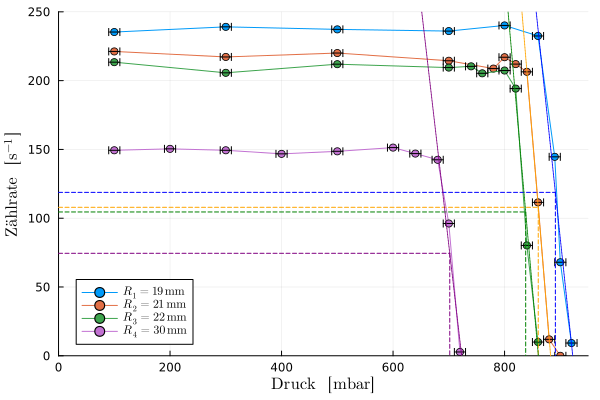
\includegraphics[width=0.9\textwidth]{../media/B3.3/zaehlratenkurven extrapoliert.pdf}
	\caption{Extrapolierte Zählratenkurven für vier Reichweiten\\
			gestrichelte Linien: $\bar r_{R_j}$ bzw. $\bar p_{R_j}$}
	\label{fig:zählratenkurvenExtrapoliert}
\end{figure}


Der Fehler der gemessenen Zählraten $r$ ist durch den statistische Fehler bestimmt \eqref{eq:statFehler}, wobei $N$ die Anzahl an gemessenen $\alpha$--Teilchen ist. Für die verschiedenen Messwerte ist er in Tabelle \ref{table_statistische_fehler} dargestellt.

Da dieser Fehler aufgrund der hohen Anzahl an gezählten $\alpha$-Teilchen sehr gering ausfällt, wird er in den folgenden Fehlerfortpflanzungen vernachlässigt werden.

\begin{eqnarray}
	\Delta r = \frac{1}{\sqrt{N}}
	\label{eq:statFehler}
\end{eqnarray}

Die mittlere Zählrate $\bar{r}$ ist nun die Hälfte der durchschnittlichen Zählrate im ersten, nahezu konstanten Teil des Graphen. Der Fehler $\Delta \bar{r}$ wird durch die mittlere Quadradsumme der Residuen ermittelt.

Die Zählvariable $k$ beschreibt hier den letzten Messwert, der den konstanten Teil des Graphen ausmacht. Der Faktor $\frac{1}{2}$ ist notwendig, da dieser Messwert die mittlere Reichweite $\bar R$ beschreiben soll, an dessen Stelle die Strahlungsintensität die Hälfte ihres Maximums erreicht.\footnote{Diese Erklärung fehlt im Abschnitt \ref{reichweite-von-alpha-teilchen}}

\begin{eqnarray}
	\bar{r}_{R_j} &=& \frac{1}{2} \cdot \frac{1}{k} \sum_{i=1}^{k} r_{i,R_j} \\
	\Delta \bar{r}_{R_j} &=& \frac{1}{2} \sqrt{\frac{1}{k (k-1)} \sum_{i=1}^{k} (r_{i,R_j} - \bar{r}_{R_j})^2}
\end{eqnarray}

Aus den mittleren Zählraten $\bar r$ sowie den Geradengleichungen mit Steigungen $a_{R_j}$ und $r$-Achsenabschnitten $b_{R_j}$ lassen sich die mittleren Drücke $\bar{p}_{R_j}$ bestimmen. Deren Fehler $\Delta \bar p_{R_j}$ werden mittels Gauß'scher Fehlerfortpflanzung ermittelt.
\begin{eqnarray}
	\bar{p}_{R_j} &=& \frac{\bar{r}_{R_j} - b_{R_j}}{a_{R_j}} \\
	\Delta \bar{p}_{R_j} &=& \sqrt{\left(\frac{\Delta \bar{r}_{R_j}}{a_{R_j}}\right)^2 + \left(\frac{\Delta b_{R_j}}{a_{R_j}}\right)^2 + \left(\frac{(\bar{r}_{R_j} - b_{R_j}) \cdot \Delta a_{R_j}}{a_{R_j}^2}\right)^2}
\end{eqnarray}

Die Abstände liefern die zugehörigen mittleren Reichweiten und damit die vier Wertepaare für mittlere Reichweite $\bar{R}$ und inversem mittlerem Druck $\frac{1}{\bar{p}}$. Die Ergebnisse sind in Tabelle \ref{table_messwerte_zählrate} zu dargestellt.

\begin{table}[H]
	\centering
	\begin{tabular}{||c|c|c|c|c||}
		\hline
		Messwert & \multicolumn{4}{c||}{$\Delta r$ [$10^{-3} \mathrm{\, 1/s}$]} \\
		\hline
		& $R_1$ & $R_2$ & $R_3$ & $R_4$ \\
		\hline \hline
		1 & 11.90 & 12.28 & 12.50 & 10.56\\
		\hline
		2 & 11.81 & 12.39 & 12.73 & 10.53\\
		\hline
		3 & 11.85 & 12.31 & 12.54 & 10.56\\
		\hline
		4 & 11.88 & 12.47 & 12.61 & 10.66\\
		\hline
		5 & 11.78 & 12.64 & 12.59 & 10.59\\
		\hline
		6 & 11.98 & 12.39 & 12.74 & 10.49\\
		\hline
		7 & 10.74 & 12.54 & 12.68 & 10.65\\
		\hline
		8 & 12.78 & 12.71 & 13.10 & 10.82\\
		\hline
		9 & 29.97 & 12.23 & 14.42 & 13.17\\
		\hline
		10 & -- & 26.41 & 28.86 & 54.88\\
		\hline
		11 & -- & n.e. & -- & --\\
		\hline
	\end{tabular}
	\caption{Statistische Fehler der gemessenen Zählraten\\
		n.e. nicht ermittelbar, da $N = 0$}
	\label{table_statistische_fehler}
	\vspace{12pt}

	\begin{tabular}{||c|c|c|c|c|c|c||}
		\hline
		$R_j$ $[\mathrm{mm}]$
			& $a_{R_j}\ [s^{-1}]$
			& $b_{R_j}\ [10^3 s^{-1}]$
			& $k$
			& $\bar{r}\ [s^{-1}]$
			& $\bar{p}\ [\mathrm{mbar}]$ \\
		\hline \hline
		$19$
			& $-3.81 \pm 0.46$
			& $3.51 \pm 0.40$
			& $5$
			& $118.77 \pm 1.81$
			& $891.14 \pm 150.55$ \\
		\hline
		$21$
			& $-4.86 \pm 0.07$
			& $4.29 \pm 0.05$
			& $7$
			& $107.90 \pm 5.42$
			& $860.42 \pm \ 16.83$ \\
		\hline
		$22$
			& $-4.60 \pm 0.63$
			& $3.96 \pm 0.53$
			& $7$
			& $104.53 \pm 3.84$
			& $837.89 \pm 162.94$ \\
		\hline
		$30$
			& $-3.49 \pm 0.68$
			& $2.52 \pm 0.47$
			& $7$
			& $\ 74.48 \pm 2.00$
			& $701.71 \pm 192.92$ \\
		\hline
	\end{tabular}
	\caption{Ergebnisse aus Zählratenkurven}
	\label{table_messwerte_zählrate}
\end{table}

\hypertarget{bestimmung-durch-Spannung}{%
	\subsubsection{Abhängigkeit von der Spannung}\label{bestimmung-durch-Spannung}}

Der eingestellte Abstand $R$ entspricht genau dann der mittleren Reichweite $\bar{R}$, wenn der Impuls $\vec{p}$ der $\alpha$-Teilchen verschwunden ist. Das Oszilloskop zeigt eine Spannung $U$ an, die proportional zum Betrag des  Impulses der $\alpha$-Teilchen ist. Die gesuchten mittleren Drücke $\bar{p}$ sind daher die Nullstellen der Kurven.
\begin{eqnarray}
	U &\propto& \lvert \vec{p}\, \rvert
\end{eqnarray}

Dafür werden die Messwerte der Spannungs-Druck Messung aufgetragen und die Enden linear gefittet, siehe Abbildung \ref{fig:spannungskurveExtrapoliert}. Die Nullstellen dieser Geraden mit Steigungen $a_{R_j}$ und $U$-Achsenabschnitten $b_{R_j}$ liefern dann die mittleren Drücke für die vier Messwertpaare für Reichweite $\bar{R}$ und inversem Druck $\frac{1}{\bar{p}}$.

Die Fehler $\Delta  \bar p_{R_j}$ werden wieder mittels Gauß'scher Fehlerfortpflanzung bestimmt. Die Ergebnisse sind in Tabelle \ref{table_messwerte_spannung} dargestellt.

\begin{eqnarray}
\bar{p}_{R_j} &=& - \frac{b_{R_j}}{a_{R_j}} \\
	\Delta \bar{p}_{R_j} &=& \sqrt{\left(\frac{\Delta b_{R_j}}{a_{R_j}}\right)^2 + \left(\frac{b_{R_j} \cdot \Delta a_{R_j}}{a_{R_j}^2}\right)^2}
\end{eqnarray}

\begin{figure}[H]
	\centering
	\includegraphics[width=0.9\textwidth]{../media/B3.3/spannungskurven extrapoliert.pdf}
	\caption{Extrapolierte Spannungskurven für vier Reichweiten \\
		gepunktete Linien: lineare Fits}
	\label{fig:spannungskurveExtrapoliert}
\end{figure}

\begin{table}[H]
	\centering
	\begin{tabular}{||c|c|c|c||}
		\hline
		$R_i\ [\mathrm{mm}]$
			& $a_{R_j}\ [\mathrm{V}]$
			& $b_{R_j}\ [\mathrm{V}]$
			& $\bar{p}\ [\mathrm{mbar}]$ \\
		\hline \hline
		$19$
			& $-0.015 \pm 0.001$
			& $14.450 \pm 1.080$
			& $956.04 \pm 105.88$ \\
		\hline
		$21$
			& $-0.013 \pm 0.002$
			& $11.390 \pm 1.291$
			& $911.20 \pm 150.39$ \\
		\hline
		$22$
			& $-0.015 \pm 0.001$
			& $13.611 \pm 0.514$
			& $883.51 \pm 49.13$ \\
		\hline
		$30$
			& $-0.017 \pm 0.001$
			& $13.072 \pm 0.781$
			& $750.69 \pm 67.42$ \\
		\hline
	\end{tabular}
	\caption{Entnommene Messwerte aus Spannungskurven}
	\label{table_messwerte_spannung}
\end{table}

\hypertarget{Reichweite-Ergebnisse}{%
	\subsubsection{Reichweitenbestimmung}\label{Reichweite-Ergebnisse}}

Die Ergebnisse aus beiden Messungsarten werden nun gegeneinander aufgetragen. Dann wird jeweils eine Geradenanpassung nach der Methode der kleinsten Fehlerquadrate durchgeführt.

Daraufhin die Geraden in $\bar R$--Richtung verschoben werden, um den Offset $R_\mathrm{off}$ der Messskala abzuziehen. Das Ergebnis ist in Abbildung \ref{fig:reichweiteInverserDruck} dargestellt.

Nun kann die Reichweite der $\alpha$-Teilchen in Luft bestimmt werden, indem der Wert Normaldruck ermittelt wird. Der Fehler wird erneut durch die Gauß'sche Fehlerfortpflanzung bestimmt, der Fehler des Normaldrucks wird als Rundungsfehler angenommen. Die Ergebnisse sind in Tabelle \ref{table_reichweite_druck} ersichtlich.

\begin{eqnarray}
	R_\mathrm{off} &=& (21.4025 \pm 1.0054) \mathrm{\,mm} \\
	\bar{R}_\mathrm{Luft} &=& a \cdot \frac{1}{\bar{p}_\mathrm{Luft}} \\
	\Delta \bar{R}_\mathrm{Luft} &=& \sqrt{\left(\frac{\Delta a}{\bar{p}_\mathrm{Luft}}\right)^2 + \left(\frac{a \cdot \Delta \bar{p}_\mathrm{Luft}}{\bar{p}_\mathrm{Luft}^2}\right)^2} \label{eq:Reichweite Luft} \\
	p_\mathrm{Luft} &=&(1013.25 \pm 0.005) \mathrm{\, mbar}
\end{eqnarray}

\begin{figure}[h!]
	\centering
	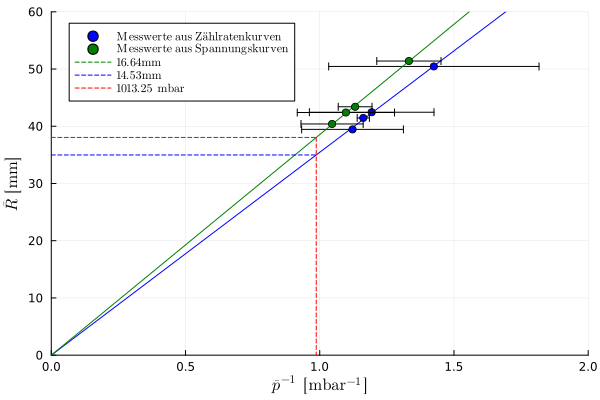
\includegraphics[width=0.9\textwidth]{../media/B3.3/reichweiten inverse druecke verschoben skaliert.pdf}
	\caption{Reichweiten gegen inverse Drücke aufgetragen}
	\label{fig:reichweiteInverserDruck}
\end{figure}

\begin{table}[H]
	\centering
	\begin{tabular}{||c|c|c||}
		\hline
		& $a\ \left[\mathrm{mm\cdot mbar}\right]$ & Reichweite in Luft $\bar{R}$ [mm]\\
		\hline \hline
		Zählratenkurven
			& $35.45 \pm 1.33$
			& $34.99 \pm 1.32$ \\
		\hline
		Spannungskurven
			& $38.55 \pm 0.87$
			& $38.04 \pm 0.88$ \\
		\hline
	\end{tabular}
	\caption{Reichweite in Luft}
	\label{table_reichweite_druck}
\end{table}

\hypertarget{Reichweite-Vergleich}{%
	\subsubsection{Vergleich der Messmethoden}\label{Reichweite-Vergleich}}

Beide Messmethoden liefern ähnliche Ergebnisse, der relative Fehler zwischen ihnen liegt bei $8.02\%$. Dies lässt sich erklären, indem man die möglichen Fehlerquellen der Methoden vergleicht.

Obwohl das Oszilloskop einen deutlich größeren Fehler aufzeigt, ist damit gut erkennbar, ob noch ein Signal gemessen wurde. Auch wenn das eintreffende Signal schwach ist, lässt es sich durch das Vergrößern der Messkurve klar erkennen.

Die Zählschwelle des $\ce{Si}$-Oberflächen-Sperrschichtzählers hingegen ist nicht so durchschaubar. Es ist durchaus möglich, dass Teilchen nicht gezählt wurden, weil ihre Restenergie zu gering war.

Daher wird in weiteren Betrachtungen die durch die Spannung gemessene mittlere Reichweite in Luft $\bar R$ verwendet werden.

Da der Unterschied zwischen den beiden Reichweitenmessungen klein ist, sind beide Methoden zufriedenstellend.

\hypertarget{Reichweite-Aluminium}{%
	\subsubsection{Reichweite in Aluminium}\label{Reichweite-Aluminium}}

Mit der nun bekannten Reichweite der $\alpha$-Teilchen in Luft lässt sich die Reichweite in Aluminium $R_\mathrm{Al}$ mit der empirischen Bragg-Kleemann-Gleichung für Luft bei $15\mathrm{\,^\circ C}$ und $1013.25 \mathrm{\, mbar}$ Mit einem Fehler $\Delta \bar{R}_\mathrm{Al}$ mittels Gauß'scher Fehlerfortpflanzung bestimmen.
\begin{eqnarray}
	\bar{R}_\mathrm{Al} &=& 3.2 \cdot 10^{-4} \mathrm{\frac{g}{cm^3}}
		\cdot \frac{A_\mathrm{Al}^{1/2}}{\rho_\mathrm{Al}} \bar{R}_\mathrm{Luft} \\
	\Delta \bar{R}_\mathrm{Al} &=& 3.2 \cdot 10^{-4} \mathrm{\frac{g}{cm^3}} \cdot
		\sqrt{
				\left(\frac{A_\mathrm{Al}^{1/2}}{\rho_\mathrm{Al}^2}\bar{R}_\mathrm{Luft} \cdot \Delta \rho_\mathrm{Al} \right)^2
				+ \left( \frac{A_\mathrm{Al}^{1/2}}{\rho_\mathrm{Al}} \Delta \bar{R}_\mathrm{Luft}\right)^2
		}
\end{eqnarray}

Für stabiles Aluminium bei Raumtemperatur hat folgende Eigenschaften, \cite{NIST_Al} woraus sich die Reichweite ergibt.

\begin{eqnarray}
	A_\mathrm{Al} &=& 27 \\
	\rho_\mathrm{Al} &=& (2.69890 \pm 0.00005) \mathrm{\frac{g}{cm^3}} \\
	\Rightarrow \bar{R}_\mathrm{Al} &=& (23.43 \pm 0.54) \mathrm{\, \mu m}
\end{eqnarray}

Der Literaturwert für die Reichweite von $\alpha$-Teilchen in Aluminium mit $4 \mathrm{\, MeV}$ beträgt $16 \mathrm{\, \mu m}$ und von $\alpha$-Teilchen mit $6 \mathrm{\, MeV}$ $30 \mathrm{\, \mu m}$. \cite{LEIFIphysik Alphazerfall }

Unsere $\alpha$-Teilchen haben eine Energie von ca. $5.5 \mathrm{\, MeV}$. Nehmen wir hier an, die Literaturwerte zwischen $4 \mathrm{\, MeV}$ und $6 \mathrm{\, MeV}$ steigen linear an. Daraus kann die Steigung $a_\mathrm{lit}$ der Literaturwerte ebenso bestimmt werden. Damit kann ein Literaturwert  $\bar R_\mathrm{lit}$ für $5.5 \mathrm{\, MeV}$ ermittelt werden.

\begin{eqnarray}
	a_\mathrm{lit} &=& 12 \mathrm{\, \frac{\mu m}{MeV}} \\
	\bar R_\mathrm{lit} &=& 24 \mathrm{\, \mu m}
\end{eqnarray}

Unser Ergebnis von $(23.43 \pm 0.54) \mathrm{\, \mu m}$ liegt innerhalb der Fehlergrenzen sehr nah an diesem Literaturwert. Dadurch lässt sich schließen, dass dieser Teil des Experiments äußerst erfolgreich verlief.

\hypertarget{energiestraggling-1}{%
	\subsection{Energiestraggling}\label{energiestraggling-1}}

\hypertarget{energiestraggling-aufloesung}{%
	\subsubsection{Auflösung}\label{energiestraggling-aufloesung}}
Die Energie $E$ in $\mathrm{keV}$ kann durch eine lineare Relation aus der Kanalnummer $K_E$ ermittelt werden. Weiterhin kann die Halbwertsbreite $\Delta E$ abgelesen werden. Nach der Annahme, dass das Straggling bei dem vorliegenden Luftdruck vernachlässigbar ist, stimmt $\Delta E$ nach Gleichung \eqref{eq:straggling parameter} mit der Auflösung $\alpha_\mathrm{res}$ des Detektors überein.

\begin{eqnarray}
	E &=& 0.525 \mathrm{\frac{keV}{Kanal }} \cdot K_E \label{eq:Kanal zu Energie}\\
	\Delta E &=& (61.9 \pm 1.2) \mathrm{\,keV} \label{eq:Halbwertsbreite} \\
	\alpha_\mathrm{res} = \frac{\Delta E}{E_\alpha} &=& (1.13 \pm 0.02) \%
\end{eqnarray}

\hypertarget{energiestraggling-straggling}{%
	\subsubsection{Straggling}\label{energiestraggling-straggling}}
Die Energiepeaks $\hat E$ und Halbwertbreiten $\Delta E$ des gemessenen $\alpha$-Spektrums sind in Tabelle \ref{tabelle: Straggling} aufgelistet.
\begin{table}
	\centering
	\begin{tabular}[h]{||c|c|c||}
		\hline
		Druck $p$ $[\mathrm{mbar}]$ & Peak $\hat E$ $[\mathrm{keV}]$ & Halbwertsbreite $\Delta E$ $[\mathrm{keV}]$  \\
		\hline\hline
		$\ 1.2 \pm 0.1$ & $5486.0 \pm 0.6$ & $\ 61.9 \pm 1.2$ \\
		\hline
		$100 \pm 10$ & $4885.6 \pm 0.6$ & $\ 79.2 \pm 1.3$ \\
		\hline
		$200 \pm 10$ & $4387.2 \pm 0.7$ & $\ 93.3 \pm 1.4$ \\
		\hline
		$300 \pm 10$ & $3862.1 \pm 1.0$ & $109.4 \pm 2.0$ \\
		\hline
		$400 \pm 10$ & $3187.4 \pm 0.9$ & $130.9 \pm 1.7$ \\
		\hline
		$500 \pm 10$ & $2603.3 \pm 1.1$ & $145.2 \pm 2.3$ \\
		\hline
		$600 \pm 10$ & $1885.6 \pm 1.3$ & $164.4 \pm 2.7$ \\
		\hline
		$700 \pm 10$ & $1088.9 \pm 1.6$ & $209.9 \pm 3.1$ \\
		\hline
		$750 \pm 10$ & $\ 670.8 \pm 1.9$ & $215.0 \pm 4.0$ \\
		\hline
		$800 \pm 10$ & $\ 226.5 \pm 3.4$ & $239.0 \pm 7.0$ \\
		\hline
	\end{tabular}
	\caption{Energie--Straggling}
	\label{tabelle: Straggling}
\end{table}

Um die Veränderung des Stragglings zu bewerten, muss zunächst die Dichte $\rho$ ermittelt werden. Diese ist über eine Referenzdichte $\rho_0$ und einen Referenzdruck $p_0$ linear vom Druck $p$ abhängig.  Dies folgt aus dem idealen Gasgesetz.

Als Referenzgröße werden Werte der Standardatmosphäre verwendet, also eine Dichte $\rho_0$ bei Normaldruck $p_0$.\footnote{FEHLER: $\rho_0$ um Faktor $10^3$ höher!} \cite{DWD}

\begin{eqnarray}
	\rho &=& \frac{\rho_0}{p_0} \cdot p \\
	\rho_0 &=& 1.225 \cdot 10^{-3}\mathrm{\,\frac{g}{cm^3}} \label{eq:Normaldichte Luft} \\
	p_0 &=& 1013.25 \mathrm{\,mbar} \label{eq:Normaldruck Luft}
\end{eqnarray}

Für den Abstand $x$ zwischen Detektor und Quelle muss der Offset $R_\mathrm{off}=(21.4025 \pm 1.0054) \mathrm{\,mm}$ berücksichtigt werden, der in Abschnitt \ref{Reichweite-Ergebnisse} ermittelt wurde. Dieser muss zu dem in der Messung abgelesenen Abstand $d=(18\pm0.5)\mathrm{\,mm}$ addiert werden, um den Abstand $x$ zu erhalten. Der Fehler für $\rho \cdot x$ ergibt sich durch Gauß'sche Fehlerfortpflanzung.

\begin{eqnarray}
	x &=& d-b\\
	x &=& (3.94025 \pm 0.10054)\mathrm{\,cm} \\
	\Delta (\rho \cdot x) &=& \sqrt{
			\left(\frac{\rho _0 \cdot x \cdot \Delta p}{p_0}\right)^2
			+ \left(\frac{\rho _0 \cdot p \cdot \Delta x}{p_0}\right)^2
		}
\end{eqnarray}

Aus dem Straggling $\alpha$ können wir den Energiestraggling-Parameter oder auch das korrigierte Straggling $\alpha_E$ nach Gleichung \eqref{eq:straggling parameter} bestimmen. Hierbei ist Energieauflösung $\alpha _\mathrm{res}$ mit der Halbwertbreite \eqref{eq:Halbwertsbreite} identisch, die bei der Eichung gemessen wurde. Die so erhaltenen Ergebnisse sind in Tabelle \ref{tabelle:korr. Straggling} dargestellt.

\begin{eqnarray}
	\alpha _E&=& \sqrt{\alpha ^2 - \alpha_\mathrm{res}^2} \\
	\Delta \alpha _E&=& \sqrt{
		\frac{(\alpha\cdot\Delta\alpha)^2}{\alpha ^2 - \alpha_\mathrm{res}^2}
		+ \frac{(\alpha_\mathrm{res} \cdot \Delta \alpha_\mathrm{res})^2}{\alpha ^2 - \alpha_\mathrm{res}^2}^2
	}
\end{eqnarray}

\begin{table}
	\centering
	\begin{tabular}[h]{||c|c|c|c||}
		\hline
		Druck $p$ $[\mathrm{mbar}]$
			& $\rho \cdot x$ $\left[10^{-3} \mathrm{\frac{g}{cm^2}}\right]$
			& $\alpha$ $[\mathrm{keV}]$ & $\alpha _E$ $[\mathrm{keV}]$\\
		\hline\hline
		$\ 1.2 \pm 0.1$ & $0.0057 \pm 0.0005$ & $\ 61.9 \pm 1.2$ & $\ \ 0.0 \pm 0.0$\\
		\hline
		$100 \pm 10$ & $0.47 \pm 0.05$ & $\ 79.2 \pm 1.3$ & $\ 49.4 \pm 2.6$  \\
		\hline
		$200 \pm 10$ & $0.95 \pm 0.05$ & $\ 93.3 \pm 1.4$ & $\ 69.8 \pm 2.2 $ \\
		\hline
		$300 \pm 10$ & $1.43 \pm 0.06$ & $109.4 \pm 2.0$ & $\ 90.2 \pm 2.6$\\
		\hline
		$400 \pm 10$ & $1.91 \pm 0.07$ & $130.9 \pm 1.7$ & $115.3 \pm 2.0$ \\
		\hline
		$500 \pm 10$ & $2.38 \pm 0.08$ & $145.2 \pm 2.3$ & $131.3 \pm 2.6$\\
		\hline
		$600 \pm 10$ & $2.86 \pm 0.09$ & $164.4 \pm 2.7$ & $152.3 \pm 3.0$ \\
		\hline
		$700 \pm 10$ & $3.33 \pm 0.10$ & $209.9 \pm 3.1$ & $200.6 \pm 3.3$ \\
		\hline
		$750 \pm 10$ & $3.57 \pm 0.10$ & $215.0 \pm 4.0$ & $205.9 \pm 4.2$\\
		\hline
		$800 \pm 10$ & $3.81 \pm 0.11$ & $239.0 \pm 7.0$ & $230.8 \pm 7.3$\\
		\hline
	\end{tabular}
	\caption{Straggling $\alpha$ und korrigiertes Straggling $\alpha_E$}
	\label{tabelle:korr. Straggling}
\end{table}

Wie man anhand der Abbildungen \ref{abb:Straggling} und \ref{abb:korr. Straggling}  erkennen kann, weisen die Graphen einen linearen Verlauf auf. Dagegen wird eine Abnahme des Energiestraggling-Parameters bei kleineren Energien erwartet. \cite{Prior}

\begin{figure}[h]
	\centering
	\includegraphics[width=0.9\textwidth]{../media/B3.3/Straggling.jpg}
	\caption{Energiestraggling $\alpha$ als Funktion von $\rho \cdot x$}
	\label{abb:Straggling}
\end{figure}

\begin{figure}[h]
	\centering
	\includegraphics[width=0.9\textwidth]{../media/B3.3/Straggling corrected.jpg}
	\caption{korrigiertes Energiestraggling $\alpha _E$ als Funktion von $\rho \cdot x$}
	\label{abb:korr. Straggling}
\end{figure}

Für eine Energieverteilung mit der Halbwertbreite von ab $10\%$ der mittleren Energie dominieren die nicht-statistischen Effekte über die statistische und das Straggling nimmt ab, d.h. das $\alpha$-Spektrum sollte ab einem bestimmen Energiewert mit abnehmender Energie bzw. zunehmendem Druck schmaler werden.

Dies lässt sich jedoch in der Auswertung nicht beobachten, weil wir zu geringen Energien haben. Um diesen Effekt beobachten zu können ist es notwendig die $10\%$ zu erreichen, dann erhält man den beschriebenen Verlauf.

Der Abstand zwischen Quelle und Detektor beträgt bei Prior bei $5\mathrm{\,cm}$  \cite{Prior}, bei uns dagegen ca. $4\mathrm{\,cm}$, möglicherweise kann unsere Abweichung damit begründet werden. Dies sei bei Laborberichten von Studenten sehr häufig der Fall. \cite{Prior} In unserem Versuchsaufbau war der Offset nicht im Voraus bekannt. Dadurch war es uns nicht möglich, einen mit Prior gut vergleichbaren Abstand einzustellen.

\hypertarget{massenbremsvermuxf6gen}{%
\subsection{Massenbremsvermögen}\label{massenbremsvermuxf6gen}}

Zuletzt soll das Massenbremsvermögen von Gold relativ zu Luft bzw. Aluminium sowie die Dicke der Aluminiumfolie bestimmen. Das relative Massenbremsvermögen $Q_F$ eines Stoffes $F$ relativ zur Luft $L$ wie folgt zu bestimmen. Dazu ist die Dichte der Luft $\rho_L$ bei den Drücken der Messungen ohne Folie $\bar p_1$ und mit Folie $\bar p_2$ bei der selben Reichweite $\bar R_1$ notwendig, ebenso wie Dichte $\rho_F$ und Dicke $d_F$ der Folie. Der Fehler wird mittels Gauß'scher Fehlerfortpflanzung bestimmt.\footnote{Fehlt ggf. in Vorbereitung, \cite[p. 5]{Uni}}

\begin{eqnarray}
	Q_F &=& \frac{\rho_L(\bar{p}_1) - \rho_L(\bar{p}_2)}{\rho_F d_F} \bar{R}_1
	\label{eq:Q_F} \\
	\Delta Q_F &=& Q \cdot \sqrt{\frac{{\Delta \rho_L(\bar{p}_1)}^2 + {\Delta \rho_L(\bar{p}_2)}^2}{\left(\rho_L(\bar{p}_1) - \rho_L(\bar{p}_2)\right)^2} + \left(\frac{\Delta \bar{R}_1}{\bar{R}_1}\right)^2 + \left(\frac{\Delta \rho_F}{\rho_F}\right)^2 + \left(\frac{\Delta d_F}{d_F}\right)^2}
\label{eq:fehler_Q_F}
\end{eqnarray}

Aus der gleichen Relation lässt sich auch die Dicke $d_F$ der Aluminiumfolie bestimmen, ebenso wie ihr Fehler.

\begin{eqnarray}
	d_F &=& \frac{\rho_L(\bar{p}_1) - \rho_L(\bar{p}_2)}{\rho_F Q_F} \bar{R}_1 \label{eq:d_F} \\
	\Delta d_F &=& d_F \cdot
		\sqrt{\frac{{\Delta \rho_L(\bar{p}_1)}^2 + {\Delta \rho_L(\bar{p}_2)}^2}{\left(\rho_L(\bar{p}_1) - \rho_L(\bar{p}_2)\right)^2} + \left(\frac{\Delta \bar{R}_1}{\bar{R}_1}\right)^2 + \left(\frac{\Delta \rho_F}{\rho_F}\right)^2 + \left(\frac{\Delta Q_F}{Q_F}\right)^2}
	\label{eq:fehler_d_F}
\end{eqnarray}

Der mittlere Druck $\bar{p}_2$ und die mittlere Reichweite $\bar{R}_1$ werden aus den Zählraten ermittelt. Dazu werden analog zum Abschnitt \ref{bestimmung-durch-zuxe4hlraten} die mit Folie gemessenen Zählraten gegen die Drücke aufgetragen und die Enden als Gerade  gefittet. Dies ist in Abbildung \ref{fig:zählraten mit folien} dargestellt.

Daraus werden erneut Wertepaare von mittlerem Druck und mittlerem Abstand bestimmt, wobei die Abstände um den Offset von $(21.40 \pm 1.01) \mathrm{\, mm}$ verschoben werden. Die Ergebnisse sind in Tabelle \ref{table_mittlereDrücke_mitFolie} ersichtlich. Diese Werte sind in Abbildung \ref{fig:reichweiteDrückeFolie} gegeneinander aufgetragen.

\begin{figure}[H]
	\centering
	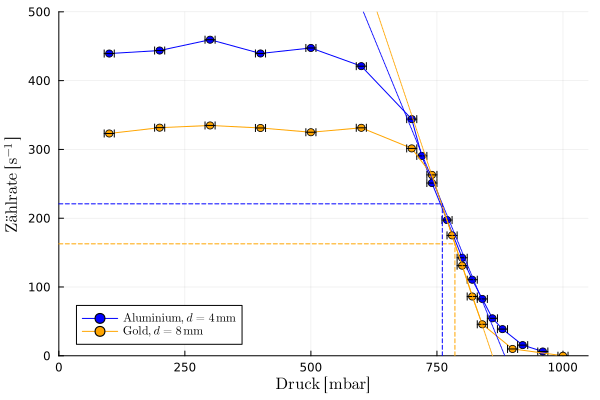
\includegraphics[width=0.7\textwidth]{../media/B3.3/zaehlraten.pdf}
	\caption{Zählratenkurven für Messung mit Aluminium- und Goldfolie \\
			gestrichelte Linien stellen mittlere Zählraten bzw. Drücke dar}
	\label{fig:zählraten mit folien}
\end{figure}

\begin{table}[H]
	\centering
	\begin{tabular}{||c||c|c||}
		\hline
		& Gold & Aluminium \\
		\hline \hline
		$\bar{p}_2$ [mbar] & $785.66 \pm 148.83$ & $760.65 \pm 219.86$ \\
		\hline
		$\bar{R}_1$ [mm] & $29.40 \pm 1.01$ & $25.40 \pm 1.01$\\
		\hline
	\end{tabular}
	\caption{Entnommene Messwertpaare aus mittlerem Druck $\bar{p}$ und mittlerer Reichweite $\bar{R}$ für Gold und Aluminium}
	\label{table_mittlereDrücke_mitFolie}
\end{table}

\begin{figure}[H]
	\centering
	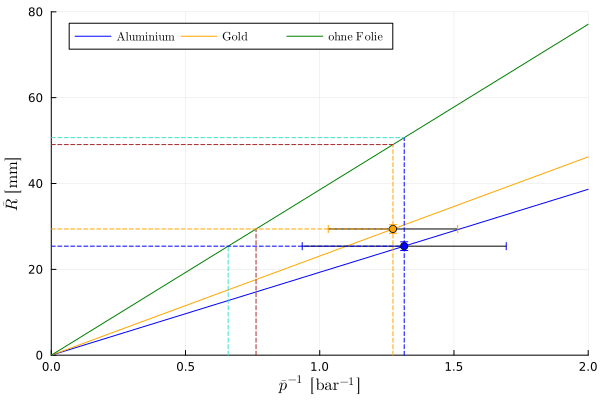
\includegraphics[width=0.7\textwidth]{../media/B3.3/reichweiten inverse druecke mit Folien.pdf}
	\caption{Reichweiten gegen inverse Drücke aufgetragen}
	\label{fig:reichweiteDrückeFolie}
\end{figure}

$\bar{p}_1$ ist der Druck aus der Messung ohne Folien, bei dem die Reichweite $\bar R(\bar p_1)$ mit der Reichweite mit Folien $\bar{R}_1$ übereinstimmt. Daher kann er aus Gleichung \eqref{eq:Reichweite Luft} hergeleitet werden, wobei die Steigung $a$ aus der Messung über die Spannung in Abschnitt \ref{Reichweite-Ergebnisse} gewählt wird. Der Fehler wird wieder über die Gauß'sche Fehlerfortpflanzung ermittelt.

\begin{eqnarray}
	\bar{p}_1 &=& \frac{a}{\bar{R}_1} \\
	\Delta \bar{p}_1 &=&
		\sqrt{\left(\frac{\Delta a}{\bar{R}_1}\right)^2 + \left(\frac{a \cdot \Delta \bar{R}_1}{\bar{R}_1^2}\right)^2}
\end{eqnarray}

Die Ergebnisse sind in Tabelle \ref{table_p_1} dargestellt.
\begin{table}[H]
	\centering
	\begin{tabular}{||c||c|c||}
		\hline
		& Gold & Aluminium \\
		\hline \hline
		$\bar{p}_1$ [mbar] & $1311.08 \pm 53.70$ & $1517.53 \pm 69.12$ \\
		\hline
	\end{tabular}
	\caption{Mittlerer Druck $\bar{p}_1$ für Gold und Aluminium}
	\label{table_p_1}
\end{table}

Um die Dichten $\rho_L(\bar{p}_1)$ und $\rho_L(\bar{p}_2)$ aus den ermittelten Drücken $\bar{p}_{1/2}$ zu bestimmen, wird die thermische Zustandsgleichung idealer Gase verwendet. Dabei wird das Volumen $V$ durch den Quotient aus Masse $m$ und Dichte $\rho$ dargestellt.
\begin{eqnarray}
	p V = p \frac{m}{\rho} &=& N k_B T \\
	\Leftrightarrow \qquad \frac{p}{\rho} &=& \frac{N}{m} k_B T
\end{eqnarray}

Sowohl die Temperatur $T$, als auch das Verhältnis von Teilchenzahl $N$ zu Masse $m$ sind in diesem Versuch konstant. Damit kann die Dichte $\rho_i$ abhängig vom Druck $p_i$ bestimmt werden. Der Fehler wird durch Gauß'sche Fehlerfortpflanzung bestimmt.

Die Dichte $\rho_0$ und der Normaldruck $p_0$ werden wie in Abschnitt \ref{energiestraggling-straggling} gewählt, siehe Gleichungen \eqref{eq:Normaldichte Luft} und \eqref{eq:Normaldruck Luft}. \cite{DWD}

\begin{eqnarray}
	\frac{p_i}{\rho_i} &=& \frac{p_0}{\rho_0} \\
	\Leftrightarrow \quad \rho_i &=& p_i \frac{\rho_0}{p_0} \\
	\Delta \rho_i &=& \sqrt{\left(\frac{\rho_0 \cdot \Delta p_i}{p_0}\right)^2 + \left(\frac{p_i \cdot \Delta \rho_0}{p_0}\right)^2 + \left(\frac{p_i \cdot \rho_0 \cdot \Delta p_0}{p_0^2}\right)^2}
\end{eqnarray}

Die so bestimmten Dichten sind in Tabelle \ref{table_dichten} zu finden.

\begin{table}[h!]
	\centering
	\begin{tabular}{||c||c|c||}
		\hline
		& Gold & Aluminium \\
		\hline \hline
		$\rho_L(\bar{p}_1)$ [kg/m$^3$] & $1.58 \pm 0.06$ & $1.80 \pm 0.08$ \\
		\hline
		$\rho_L(\bar{p}_2)$ [kg/m$^3$] & $0.95 \pm 0.18$ & $0.90 \pm 0.26$ \\
		\hline
	\end{tabular}
	\caption{Dichten $\rho_L(\bar{p}_{1/2})$ für Gold und Aluminium}
	\label{table_dichten}
\end{table}

Nun werden noch die Dichten der Goldfolie $\rho_\mathrm{Au}$ \cite{DichteGold} und der Aluminiumfolie $\rho_\mathrm{Al}$ \cite{DichteAlu} benötigt, ebenso wie die Dicke der Goldfolie $d_\mathrm{Au}$ \cite{Uni} und das relative Massenbremsvermögen von Aluminium zu Luft $Q_\mathrm{Al}$ \cite{Uni}.

\begin{eqnarray}
	\rho_\mathrm{Au} &=& (19.32 \pm 0.005) \mathrm{\, \frac{g}{cm^3}}\\
	\rho_\mathrm{Al} &=& (2.6989 \pm 0.00005) \mathrm{\, \frac{g}{cm^3}}\\
	d_\mathrm{Au} &=& (2.50 \pm 0.25) \mathrm{\, \mu m}\\
	Q_\mathrm{Al} &=& (0.78 \pm 0.04)
\end{eqnarray}

Das Massenbremsvermögen von Gold zu Aluminium folgt aus den Gleichungen \eqref{eq:Q_F} und \eqref{eq:fehler_Q_F}, die Dicke der Aluminiumfolie aus den Gleichungen \eqref{eq:d_F} und \eqref{eq:fehler_d_F}.
\begin{eqnarray}
	Q_\mathrm{Au} &=& 0.38 \pm 0.12 \\
	d_\mathrm{Al} &=& (10.86 \pm 3.36) \mathrm{\, \mu m}
\end{eqnarray}

Zudem kann das relative Massenbremsvermögen von Gold zu Aluminium $Q_\mathrm{Au, Al}$ als Quotient der relativen Massenbremsvermögens von Gold zu Luft $Q_\mathrm{Au}$ bzw. von Aluminium zu Luft $Q_\mathrm{Al}$ ermittelt werden. Der Fehler wird wiederum durch Gauß'sche Fehlerfortpflanzung bestimmt.

\begin{eqnarray}
	Q_\mathrm{Au, Al} &=& \frac{Q_\mathrm{Au}}{Q_\mathrm{Al}} \\
	\Delta Q_\mathrm{Au, Al} &=&
		\sqrt{
				\left(\frac{\Delta Q_\mathrm{Au}}{Q_\mathrm{Al}}\right)^2
				+ \left(\frac{Q_\mathrm{Au}}{{Q_\mathrm{Al}}^2} \Delta Q_\mathrm{Al} \right)^2
			} \\
	\Rightarrow Q_\mathrm{Au, Al} &=& 0.49 \pm 0.16
\end{eqnarray}

\clearpage
\hypertarget{literatur}{%
\section{Literaturverzeichnis}\label{literatur}}
\renewcommand{\section}[2]{}

\begin{thebibliography}{99}
\bibitem{Bethge}
	K. Bethge, ``Kernphysik: Eine Einführung'', 3. Auflage,
	Springer-Verlag, 2008, ISBN: 9783540745679, DOI:
	\href{https://doi.org/10.1007/978-3-540-74567-9}{10.1007/978-3-540-74567-9}

\bibitem{Prior}
	Prior und Rollefson, ``Anomalous energy straggling of alpha
	particles'', American Journal of Physics, Mai 1982,
	\href{https://doi.org/10.1119/1.12834}{DOI 10.1119/1.12834}

\bibitem{Chart of Nuclides}
	``Chart of Nuclides'', National Nuclear Data Center,
	\url{https://www.nndc.bnl.gov/nudat3}, $^{241}_{\ \ 95}\mathrm{Am}$,
	Abruf am 28.01.2024

\bibitem{hdtv}
	Software \href{https://pypi.org/project/hdtv}{\texttt{hdtv}},
	Kurzanleitung unter
	\url{https://www.ikp.uni-koeln.de/fileadmin/data/praktikum/hdtv.pdf},
	Abruf am 28.01.2024

\bibitem{SpektrumOberfl.Zähler}
	Lexikon der Physik, Spektrum Verlag,
	\url{https://www.spektrum.de/lexikon/physik/oberflaechensperrschichtzaehler/10568},
	29.01.2024

\bibitem{Knoll}
	G. Knoll, ``Radiation Detection and Measurement'', Wiley, 2010, ISBN:
	9780470131480

\bibitem{Demtröder}
	W. Demtröder, ``Experimentalphysik 4: Kern-, Teilchen- und
	Astrophysik'', Springer-Spektrum-Verlag, 2017, ISBN: 9783662528839,
	DOI:
	\href{https://doi.org/10.1007/978-3-662-52884-6}{10.1007/978-3-662-52884-6}

\bibitem{Ionization Energy}
	NIH National Library of Medicine NCBI, ``Ionization Energy in the
	Periodic Table of Elements'',
	\url{https://pubchem.ncbi.nlm.nih.gov/periodic-table/ionization-energy},
	Abruf am 28.01.2024
	
\bibitem{NIST_Al}
	National Institute of Standards and Technology, ``Composition of  Aluminium'',
	\url{https://physics.nist.gov/cgi-bin/Star/compos.pl?matno=013}

\bibitem{LEIFIphysik Alphazerfall }
	LEIFIphysik, ``Alphazerfall und Alphastrahlung'',
	\url{https://www.leifiphysik.de/kern-teilchenphysik/radioaktivitaet-einfuehrung/grundwissen/alphazerfall-und-alphastrahlung},
	Abruf am 01.03.2024

\bibitem{DWD}
	DWD, ``Standardatmosphäre'',
	\url{https://www.dwd.de/DE/service/lexikon/begriffe/S/Standardatmosphaere_pdf.pdf?__blob=publicationFile}, Abruf am 10.03.2024

\bibitem{DichteGold}
	N. N. Greenwood, A. Earnshaw, ``Chemie der Elemente'', 1. Auflage, Verlag Chemie,
	ISBN 3-527-26169-9, S. 1509

\bibitem{DichteAlu}
	C. Kammer, ``Aluminium-Taschenbuch -- Band 1'', 16. Auflage, Aluminium-Verlag, Düsseldorf 2002,
	ISBN 3-410-22028-3, S. 74

\bibitem{Uni}
	Universität zu Köln, ``B3.3: Reichweite von $\alpha$-Teilchen'', Januar 2021, Online verfügbar unter \url{https://www.ikp.uni-koeln.de/fileadmin/data/praktikum/B3.3_alpha_de.pdf}

\end{thebibliography}
\end{document}
